\documentclass{article}

% ================================================================
% Idioma y codificación
% ================================================================
\usepackage[spanish]{babel}
\usepackage[T1]{fontenc}
\usepackage[utf8]{inputenc}

% ================================================================
% Gráficos y layout
% ================================================================
\usepackage{graphicx}
\graphicspath{{imagenes/}}
\usepackage[colorlinks=true, allcolors=blue]{hyperref}
\usepackage[letterpaper,top=2cm,bottom=5cm,left=3cm,right=3cm,marginparwidth=1.75cm]{geometry}

% ================================================================
% Matemáticas y símbolos
% ================================================================
\usepackage{amsmath}
\usepackage{amssymb}

% ================================================================
% Tablas y color
% ================================================================
\usepackage{tabularx}
\usepackage{array}
\usepackage{colortbl}
\usepackage{xcolor}
\definecolor{headerblue}{RGB}{30,60,120}

% ================================================================
% Listas, figuras y formato
% ================================================================
\usepackage{enumitem}
\usepackage{float}
\usepackage{subcaption}
\usepackage{fancyhdr}
\usepackage{parskip}

\pagestyle{fancy}
\fancyhf{}
\setlength{\headheight}{70pt}

% Definición del encabezado
\fancyhead[C]{%
    \begin{minipage}[c]{1.5cm}
        \includegraphics[width=1.5cm]{imagenes/uta.png}
    \end{minipage}%
    \hfill
    \begin{minipage}[c]{10cm}
        \centering
        \small {\textbf{UNIVERSIDAD TÉCNICA DE AMBATO}} \\[0.1cm]
        \scriptsize \textit{FACULTAD DE INGENIERÍA EN SISTEMAS ELECTRÓNICA E INDUSTRIAL} \\[0.1cm]
        \scriptsize \textbf{CARRERA SOFTWARE} \\[0.1cm]
        \scriptsize \textbf{CICLO ACADÉMICO: JULIO - DICIEMBRE 2026}
        \vspace{0.2cm}
    \end{minipage}%
    \hfill
    \begin{minipage}[c]{1.5cm}
        \centering
        \includegraphics[width=1.5cm]{imagenes/fisei.png}
    \end{minipage}%
}
\fancyfoot[C]{\thepage}

\begin{document}
\begin{center}
    {\large \textbf{INFORME DE GUÍA PRÁCTICA}} \\
\end{center}

% ================================================================
\section{Portada}
% ================================================================
\begin{flushleft}
\begin{tabular}{ l p{9cm} }
    \textbf{Tema:} & APE 6. Evaluación y validación --- Fases 3 y 4: Aplicación, análisis y cierre \\
    \textbf{Unidad de Organización Curricular:} & Profesional \\
    \textbf{Nivel y Paralelo:} & 5 - A \\
    \textbf{Alumnos participante(s):} & Cholota Bastidas Ariel Isai \\
                                      & García Amores Manolo José \\
                                      & Miranda Tarupi Luis Sebastián \\
                                      & Velasco Huayamave Kevin Andrés \\
    \textbf{Asignatura:} & Interacción Humano/Computador \\
    \textbf{Docente:} & Ing. Caiza Caizabuano Jose Ruben \\
\end{tabular}
\end{flushleft}

% ================================================================
\section{Informe de guía práctica}
% ================================================================

\subsection{Objetivos}
\subsubsection{General}
Ejecutar la evaluación formativa del prototipo \textbf{CaféU V2} mediante una inspección heurística independiente con severidad y una prueba de usabilidad con usuarios bajo pensamiento en voz alta, consolidar las métricas de eficacia, eficiencia y satisfacción (ISO 9241-11:2018) y cerrar la evaluación con la matriz de hallazgos, la triangulación de métodos, los criterios técnicos verificables y el backlog priorizado.

\subsubsection{Específicos}
\begin{itemize}[leftmargin=1.5em, itemsep=2pt]
    \item Revisar las brechas del pilotaje y aplicar los ajustes post-pilotaje al prototipo (versión 2).
    \item Incorporar tareas de refuerzo para evaluar buscador, filtros y prevención de errores.
    \item Definir y verificar el reinicio de estado (F5) entre sesiones.
    \item Aplicar las 10 heurísticas de Nielsen de forma independiente y calificar cada problema con severidad de 1 a 4, ponderando frecuencia, impacto y persistencia.
    \item Ejecutar sesiones individuales con tres participantes externos aplicando el consentimiento informado, los cuatro roles del laboratorio y el cuestionario SUS.
    \item Calcular la tasa de éxito autónomo, los errores críticos y no críticos, la mediana de tiempo por tarea y el puntaje SUS.
    \item Comparar los resultados con la Fase 2 y documentar los hallazgos consolidados.
    \item Consolidar los hallazgos de ambos métodos en una matriz única con severidad, prioridad y propuesta de mejora.
    \item Triangular los resultados para distinguir los hallazgos comunes de los exclusivos de cada método.
    \item Definir criterios técnicos verificables, con su estándar de respaldo y su umbral de aceptación.
    \item Priorizar el backlog y dejar los Issues trazables en GitHub, con rama, responsable y revisor.
    \item Responder la pregunta de evaluación y documentar las limitaciones del estudio.
\end{itemize}

\subsection{Modalidad}
Presencial

\subsection{Tiempo de duración}
Presenciales: 3\\
No presenciales: 2

\subsection{Instrucciones}
\textbf{Acciones previas:}
\begin{itemize}[leftmargin=1.5em, itemsep=2pt]
    \item Abrir el prototipo CaféU V2 y verificar que el encabezado muestre la marca de versión.
    \item Ejecutar el reinicio de estado (F5) y comprobar contador en cero, pedido vacío, buscador vacío, filtro «Todas» y vista Inicio.
    \item Preparar el consentimiento informado, la hoja de observación, el cronómetro y el cuestionario SUS.
    \item Confirmar los roles: moderador, usuario, cronometrista y observador; el soporte técnico controla el reinicio y la grabación.
    \item Realizar un ensayo interno con un integrante (no cuenta como dato) para probar las nueve tareas y el reinicio.
\end{itemize}

\textbf{Pasos:}
\begin{enumerate}[leftmargin=1.5em, itemsep=2pt]
    \item Aplicar el consentimiento informado y verificar el perfil del participante.
    \item Explicar la técnica de pensamiento en voz alta sin revelar las tareas.
    \item Ejecutar las nueve tareas cronometradas, con la pista única estandarizada cuando corresponda.
    \item Registrar éxito, tiempo, errores críticos y no críticos, y frases textuales.
    \item Aplicar el cuestionario SUS al finalizar cada sesión.
    \item Ejecutar F5 y verificar el estado inicial antes del siguiente participante.
    \item Consolidar las métricas ISO 9241-11 y compararlas con la Fase 2.
    \item Realizar la inspección heurística individual y consolidar las severidades.
    \item Construir la matriz consolidada y triangular los dos métodos.
    \item Definir los criterios técnicos verificables y priorizar el backlog.
    \item Documentar los hallazgos, las conclusiones y las evidencias en el repositorio.
\end{enumerate}

\subsection{Listado de equipos, materiales y recursos}
\textbf{Listado de equipos y materiales generales empleados en la guía práctica:}
\begin{itemize}[leftmargin=1.5em, itemsep=3pt]
    \item Computadora
    \item Navegador web (Chrome) y cronómetro
    \item Prototipo CaféU V2 (HTML, CSS y JavaScript)
    \item Consentimiento informado, hoja de observación y cuestionario SUS
    \item Hojas de evaluación heurística individual
    \item Herramientas ofimáticas, aula virtual e internet
    \item Visual Studio Code y GitHub
\end{itemize}

\textbf{TAC (Tecnologías para el Aprendizaje y Conocimiento) empleados en la guía práctica:}
\begin{itemize}[leftmargin=1.5em, itemsep=2pt]
    \item[$\square$] Plataformas educativas
    \item[$\square$] Simuladores y laboratorios virtuales
    \item[$\square$] Aplicaciones educativas
    \item[$\square$] Recursos audiovisuales
    \item[$\square$] Gamificación
    \item[$\blacksquare$] Inteligencia Artificial
    \item Otros (Especifique): \underline{\hspace{5cm}}
\end{itemize}

\subsection{Actividades por desarrollar}
\begin{enumerate}[leftmargin=1.5em, itemsep=2pt]
    \item \textbf{Ajuste post-pilotaje (3.1):} revisar las brechas de la Fase 2, aplicar los cambios al prototipo y definir el reinicio F5. \textbf{Producto:} prototipo V2 y documento de ajustes.
    \item \textbf{Evaluación heurística individual (3.2):} cada integrante inspecciona el prototipo con las 10 heurísticas de Nielsen y asigna severidad de 1 a 4. \textbf{Producto:} cuatro evaluaciones individuales y una consolidada.
    \item \textbf{Prueba con usuarios (3.3):} ejecutar las nueve tareas con tres participantes externos bajo pensamiento en voz alta y aplicar el SUS. \textbf{Producto:} registros P1, P2 y P3.
    \item \textbf{Métricas ISO 9241-11 (3.4):} calcular eficacia, eficiencia y satisfacción. \textbf{Producto:} resumen de métricas y comparación con la Fase 2.
    \item \textbf{Consolidación y triangulación (4.1--4.2):} fusionar los hallazgos de ambos métodos, asignar prioridad y contrastar la cobertura de cada uno. \textbf{Producto:} matriz consolidada y análisis de triangulación.
    \item \textbf{Criterios y backlog (4.3--4.4):} definir criterios verificables con su estándar y convertir los hallazgos en un backlog priorizado. \textbf{Producto:} criterios C-01 a C-09 y backlog P1--P4.
    \item \textbf{Cierre y colaboración (4.5):} responder la pregunta de evaluación y preparar los Issues, ramas y Pull Requests. \textbf{Producto:} conclusiones, 9 Issues y plan de colaboración.
\end{enumerate}

\subsection{Resultados obtenidos}

\subsubsection{Antecedentes: Fases 1 y 2}
En la Fase 1 se planificó la evaluación de usabilidad de \textbf{CaféU}, una aplicación web móvil para pedir en la cafetería universitaria antes de llegar. En la Fase 2 se ejecutó el pilotaje con tres participantes (P1, P2 y P3) y seis tareas. El pilotaje obtuvo una tasa de éxito de 17/18 (94~\%), un SUS promedio de 83,3 y tres hallazgos preliminares: el botón de quitar poco visible, el buscador sin manejo de tildes y el aviso de «agregado» demasiado breve.

\subsubsection{Ajuste post-pilotaje: versión 1 a versión 2}
A partir de las brechas del pilotaje se aplicaron seis cambios al prototipo. La versión 2 conserva el catálogo, el flujo de cinco pantallas y el código de retiro \texttt{\#CU-104}.

\begin{center}
\small
\begin{tabular}{|c|p{4.4cm}|p{5.2cm}|p{3.2cm}|}
\hline
\textbf{\#} & \textbf{Brecha de la Fase 2} & \textbf{Cambio en V2} & \textbf{Verificación} \\
\hline
1 & Botón de quitar solo con el símbolo $\times$ & Botón «Quitar» con texto, papelera y \texttt{aria-label} & T4: 24 s a 17 s \\
\hline
2 & Buscador sin manejo de tildes & Normalización NFD de nombres y descripciones & T7: 3/3 \\
\hline
3 & Aviso de «agregado» borrado al navegar & Toast de 5 s con \texttt{role=status} & Sigue siendo sutil: H-01 \\
\hline
4 & Pedido vacío confirmable & Botón deshabilitado, motivo visible y guarda en la función & T9: 2/3 + 1 con ayuda \\
\hline
5 & Consigna ambigua de T6 & Consigna reformulada con acción explícita & T6: 3/3 \\
\hline
6 & Funciones críticas sin probar & Tareas de refuerzo T7, T8 y T9 & Protocolo ampliado \\
\hline
\end{tabular}
\end{center}

\textbf{Reinicio de estado (F5).} El pedido vive únicamente en memoria, por lo que recargar la página restablece la aplicación. Antes de cada sesión, el soporte técnico verifica: (1) vista Inicio visible; (2) contador del carrito en cero; (3) pedido vacío con «Confirmar» deshabilitado; (4) buscador vacío; (5) filtro «Todas» activo; (6) recorrido de humo de agregar y quitar; (7) pestaña limpia si hubo una sesión previa.

\subsubsection{Protocolo de la Fase 3: nueve tareas}
Se mantuvieron las seis tareas del pilotaje y se agregaron tres tareas de refuerzo orientadas a las funciones críticas que no se habían probado.

\begin{center}
\small
\begin{tabular}{|c|p{7.6cm}|c|p{3.4cm}|}
\hline
\textbf{ID} & \textbf{Consigna} & \textbf{Meta / Máx} & \textbf{Qué evalúa} \\
\hline
T1 & ¿En qué horario atiende la cafetería? & 60 / 120 & Consulta \\
\hline
T2 & Agrega un sánduche de queso a tu pedido. & 60 / 120 & Creación \\
\hline
T3 & Agrega también dos cafés americanos. & 60 / 120 & Modificación \\
\hline
T4 & Ya no quieres el sánduche. Quítalo, confirma tu pedido y dime tu número de pedido. & 90 / 180 & Modificación y confirmación \\
\hline
T5 & ¿Cuántos productos de comida ofrece la cafetería? & 60 / 120 & Consulta y filtros \\
\hline
T6 & Simula agregar 3 croissants a tu pedido y dime el total a pagar. & 90 / 180 & Cálculo \\
\hline
T7 & Busca un café americano escribiendo «cafe» sin tilde y agrégalo. & 60 / 120 & Buscador (refuerzo) \\
\hline
T8 & Con el filtro Comida activo, busca «café». ¿Qué ves? Llega al café americano. & 90 / 180 & Filtros y recuperación (refuerzo) \\
\hline
T9 & Abre Mi pedido sin agregar nada e intenta confirmar. Explícame qué ocurre. & 60 / 120 & Prevención de errores (refuerzo) \\
\hline
\end{tabular}
\end{center}

\subsubsection{Método 1: evaluación heurística independiente}
Cada integrante inspeccionó el prototipo por separado con las diez heurísticas de Nielsen (1994), sin ver las listas de los demás. Para cada problema se calificaron frecuencia (F), impacto (I) y persistencia (P) de 1 a 4, y se calculó la severidad como $S = \operatorname{redondeo}((F + I + P)/3)$. La severidad consensuada es la mediana de los cuatro evaluadores.

\begin{center}
\small
\begin{tabular}{|c|p{6.2cm}|c|}
\hline
\textbf{Valor} & \textbf{Nivel} & \textbf{Descripción} \\
\hline
1 & Cosmético & No afecta la tarea; se corrige si hay tiempo. \\
\hline
2 & Menor & Genera fricción breve; el usuario se recupera solo. \\
\hline
3 & Mayor & Afecta la comprensión o la eficiencia; corrección prioritaria. \\
\hline
4 & Crítico & Impide o compromete la tarea; corregir antes de liberar. \\
\hline
\end{tabular}
\end{center}

\begin{center}
\small
\begin{tabular}{|c|p{5.4cm}|c|c|c|c|c|}
\hline
\textbf{ID} & \textbf{Hallazgo} & \textbf{Luis} & \textbf{Kevin} & \textbf{Manolo} & \textbf{Ariel} & \textbf{Consenso} \\
\hline
H-01 & Aviso «agregado» efímero y poco perceptible & 3 & 3 & 4 & 3 & \textbf{3} \\
\hline
H-02 & Búsqueda sin resultados no ofrece recuperación & 3 & 3 & 3 & 3 & \textbf{3} \\
\hline
H-03 & Salir de la confirmación borra el pedido sin aviso & 2 & 2 & 2 & 2 & \textbf{2} \\
\hline
H-04 & Motivo del bloqueo de «Confirmar» separado y pequeño & -- & 2 & 3 & 2 & \textbf{2} \\
\hline
H-05 & Código de retiro no copiable ni con instrucción & 2 & 2 & 1 & 2 & \textbf{2} \\
\hline
H-06 & Contador del carrito sin unidad ni etiqueta & 1 & 1 & 1 & 1 & \textbf{1} \\
\hline
H-07 & Sin indicador de pasos del flujo & 1 & -- & 1 & 1 & \textbf{1} \\
\hline
\end{tabular}
\end{center}

Los cuatro evaluadores coincidieron en H-01, H-02, H-03, H-05 y H-06. Manolo y Ariel reportaron los siete hallazgos heurísticos; Luis y Kevin, seis. La inspección se complementó con la observación de usuarios, que aportó dos hallazgos adicionales (H-08 y H-09).

\subsubsection{Método 2: prueba de usabilidad con usuarios}
Se realizaron tres sesiones individuales de 30 minutos con participantes externos, aplicando el consentimiento informado anonimizado y el pensamiento en voz alta. La pista única se leyó como máximo una vez por tarea.

\begin{center}
\small
\begin{tabular}{|c|c|c|c|c|}
\hline
\textbf{Código} & \textbf{Edad} & \textbf{Carrera} & \textbf{Semestre} & \textbf{Consentimiento} \\
\hline
P1 & 20 & Software & 5 & Aceptado \\
\hline
P2 & 21 & Sistemas & 4 & Aceptado \\
\hline
P3 & 22 & Software & 5 & Aceptado \\
\hline
\end{tabular}
\end{center}

\begin{center}
\small
\begin{tabular}{|p{3.2cm}|p{3.4cm}|p{8.4cm}|}
\hline
\textbf{Rol} & \textbf{Integrante} & \textbf{Función} \\
\hline
Moderador & Luis Miranda & Lee el consentimiento y las consignas; aplica la pista única. \\
\hline
Usuario & P1 / P2 / P3 & Ejecuta las tareas y verbaliza lo que piensa. \\
\hline
Cronometrista & Kevin Velasco & Cronometra y registra éxito, tiempos y errores. \\
\hline
Observador & Manolo García & Anota frases textuales y heurísticas afectadas. \\
\hline
Soporte técnico & Ariel Cholota & Ejecuta F5 y controla la grabación. \\
\hline
\end{tabular}
\end{center}

\subsubsection{Métricas ISO 9241-11:2018}
\textbf{Eficacia.} Se alcanzó una tasa de éxito autónomo de 26/27 ejecuciones (96,3~\%), sin errores críticos y con tres errores no críticos recuperados por los propios participantes.

\begin{center}
\scriptsize
\begin{tabular}{|c|c|c|c|c|c|c|c|c|}
\hline
\textbf{Tarea} & \textbf{Meta} & \textbf{P1} & \textbf{P2} & \textbf{P3} & \textbf{Éxito} & \textbf{Mediana} & \textbf{Crít.} & \textbf{No crít.} \\
\hline
T1 & 60 & 5 & 7 & 6 & 3/3 & 6 & 0 & 0 \\
\hline
T2 & 60 & 12 & 14 & 13 & 3/3 & 13 & 0 & 0 \\
\hline
T3 & 60 & 19 & 21 & 18 & 3/3 & 19 & 0 & 1 \\
\hline
T4 & 90 & 16 & 19 & 17 & 3/3 & 17 & 0 & 1 \\
\hline
T5 & 60 & 7 & 9 & 8 & 3/3 & 8 & 0 & 0 \\
\hline
T6 & 90 & 14 & 17 & 15 & 3/3 & 15 & 0 & 0 \\
\hline
T7 & 60 & 12 & 14 & 13 & 3/3 & 13 & 0 & 0 \\
\hline
T8 & 90 & 15 & 24 & 18 & 3/3 & 18 & 0 & 1 \\
\hline
T9 & 60 & 8 & 13$^{*}$ & 9 & 2/3 & 9 & 0 & 0 \\
\hline
\textbf{Total} & -- & -- & -- & -- & \textbf{26/27} & -- & \textbf{0} & \textbf{3} \\
\hline
\end{tabular}
\end{center}

{\scriptsize $^{*}$ P2 completó T9 después de la pista única; no cuenta como éxito autónomo.}

\textbf{Eficiencia.} Las nueve tareas quedaron por debajo de su meta. La tarea más lenta fue T8, con 18 s de mediana.

\textbf{Satisfacción.} El SUS promedio fue 86,7 (P1 = 90,0; P2 = 77,5; P3 = 92,5), por encima de la referencia de 68,0.

\begin{center}
\small
\begin{tabular}{|c|p{7.6cm}|c|c|c|}
\hline
\textbf{N°} & \textbf{Ítem SUS (resumido)} & \textbf{P1} & \textbf{P2} & \textbf{P3} \\
\hline
1 & Me gustaría usar este sistema con frecuencia & 4 & 4 & 4 \\
\hline
2 & Encontré el sistema innecesariamente complejo & 1 & 1 & 1 \\
\hline
3 & Pensé que el sistema era fácil de usar & 5 & 4 & 5 \\
\hline
4 & Necesitaría el apoyo de un técnico & 1 & 1 & 1 \\
\hline
5 & Las funciones estaban bien integradas & 4 & 4 & 4 \\
\hline
6 & Había demasiada inconsistencia & 1 & 2 & 1 \\
\hline
7 & La mayoría aprendería a usarlo rápidamente & 5 & 4 & 5 \\
\hline
8 & Encontré el sistema muy engorroso & 2 & 2 & 1 \\
\hline
9 & Me sentí muy seguro usando el sistema & 4 & 3 & 4 \\
\hline
10 & Necesité aprender muchas cosas antes & 1 & 2 & 1 \\
\hline
\multicolumn{2}{|l|}{\textbf{Puntaje SUS ($\times$ 2,5)}} & 90,0 & 77,5 & 92,5 \\
\hline
\end{tabular}
\end{center}

\subsubsection{Comparación con la Fase 2}
\begin{center}
\small
\begin{tabular}{|p{4.6cm}|c|c|p{5.2cm}|}
\hline
\textbf{Indicador} & \textbf{Fase 2} & \textbf{Fase 3} & \textbf{Lectura} \\
\hline
Éxito autónomo & 94~\% & 96,3~\% & Se mantiene alto con tres tareas nuevas \\
\hline
T4: mediana & 24 s & 17 s & El botón «Quitar» redujo la duda \\
\hline
T6: éxito & 2/3 & 3/3 & La consigna reformulada eliminó la ambigüedad \\
\hline
SUS promedio & 83,3 & 86,7 & Mejora ligera \\
\hline
Tareas y duración & 6 / 20 min & 9 / 30 min & Incluye las tareas de refuerzo \\
\hline
\end{tabular}
\end{center}

\subsubsection{Matriz consolidada de hallazgos (Fase 4.1)}
La severidad consensuada es la mediana de los cuatro evaluadores. La prioridad combina esa severidad con la coincidencia de métodos y el impacto en las métricas ISO. Ningún hallazgo resultó crítico: los problemas están en la comunicación del estado y en la recuperación, no en el funcionamiento.

\begin{center}
\small
\begin{tabular}{|c|p{6.1cm}|c|c|c|c|}
\hline
\textbf{ID} & \textbf{Hallazgo} & \textbf{Heur.} & \textbf{Sev.} & \textbf{Prior.} & \textbf{Criterio} \\
\hline
H-01 & Aviso «agregado» efímero y poco perceptible & H1 & 3 & P1 & C-01 \\
\hline
H-02 & Búsqueda sin resultados no ofrece recuperación & H9 & 3 & P1 & C-02 \\
\hline
H-03 & Salir de la confirmación borra el pedido sin aviso & H3 & 2 & P2 & C-03 \\
\hline
H-04 & Motivo del bloqueo separado del botón & H5 & 2 & P1 & C-04 \\
\hline
H-05 & Código de retiro no copiable ni con instrucción & H10 & 2 & P2 & C-05 \\
\hline
H-06 & Contador del carrito sin unidad ni etiqueta & H1/H2 & 1 & P4 & C-06 \\
\hline
H-07 & Sin indicador de pasos del flujo & H1 & 1 & P4 & C-07 \\
\hline
H-08 & Tocar un ítem del pedido no abre el detalle & H4 & 2 & P3 & C-08 \\
\hline
H-09 & Los usuarios buscan el total desde el menú & H6 & 1 & P4 & C-09 \\
\hline
\end{tabular}
\end{center}

Distribución: 0 críticos, 2 mayores, 4 menores y 3 cosméticos. La propuesta de mejora de cada hallazgo está en \texttt{docs/matriz-consolidada.md}.

\subsubsection{Triangulación de métodos (Fase 4.2)}
De los 9 hallazgos, la inspección detectó 7 (77,8~\%), los usuarios 5 (55,6~\%) y solo 3 coincidieron (33,3~\%). La heurística encuentra riesgos latentes que el recorrido feliz no dispara; los usuarios revelan expectativas que la inspección no puede anticipar.

\begin{center}
\small
\begin{tabular}{|p{3.2cm}|p{8.4cm}|c|}
\hline
\textbf{Origen} & \textbf{Hallazgos} & \textbf{Cantidad} \\
\hline
Ambos métodos & H-01, H-02, H-04 & 3 \\
\hline
Solo heurística & H-03, H-05, H-06, H-07 & 4 \\
\hline
Solo usuarios & H-08, H-09 & 2 \\
\hline
\end{tabular}
\end{center}

Los tres hallazgos comunes son también los de mayor prioridad, lo que respalda la P1 sin depender de una sola fuente de evidencia.

\subsubsection{Criterios técnicos verificables (Fase 4.3)}
Cada hallazgo tiene un criterio observable, un estándar de respaldo y un umbral de aceptación. Un Issue no se cierra sin evidencia de su cumplimiento.

\begin{center}
\scriptsize
\begin{tabular}{|c|p{4.3cm}|p{4.6cm}|p{4.2cm}|}
\hline
\textbf{ID} & \textbf{Criterio} & \textbf{Estándar} & \textbf{Umbral} \\
\hline
C-01 & El usuario percibe que el producto se agregó & ISO 9241-110; WCAG 4.1.3 y 1.4.3 & 3/3 sin mirar el contador; 5 s; 4,5:1 \\
\hline
C-02 & Entiende el vacío y puede salir & ISO 9241-110; WCAG 3.3.1 y 3.3.3 & 3/3 en 10 s o menos, sin pista \\
\hline
C-03 & Salir de la confirmación no destruye el pedido & ISO 9241-110; WCAG 3.3.1 & 0 pérdidas silenciosas \\
\hline
C-04 & Comprende por qué no puede confirmar & WCAG 3.3.1, 3.3.3 y 1.4.1 & 3/3 en 5 s o menos; motivo adyacente \\
\hline
C-05 & Copia el código y sabe para qué sirve & ISO 9241-110; Nielsen H10 & Un clic e instrucción de uso \\
\hline
C-06 & El contador comunica cantidad y unidad & WCAG 4.1.2 & Nombre accesible con unidad \\
\hline
C-07 & Sabe en qué paso del flujo está & WCAG 2.4.8; ISO 9241-110 & Indicador visible y \texttt{aria-current} \\
\hline
C-08 & El ítem del pedido abre su detalle & ISO 9241-110; WCAG 3.2.4 & 0 controles muertos \\
\hline
C-09 & El total se ve sin abrir el pedido & ISO 9241-110; Nielsen H6 & 3/3 lo leen desde el menú \\
\hline
\end{tabular}
\end{center}

\subsubsection{Backlog priorizado (Fase 4.4)}
Los nueve hallazgos se agruparon en cuatro prioridades, con un esfuerzo total estimado de 22 horas y una iteración por grupo.

\begin{center}
\small
\begin{tabular}{|c|c|c|c|p{5.2cm}|}
\hline
\textbf{Prior.} & \textbf{Hallazgos} & \textbf{Esf.} & \textbf{Iter.} & \textbf{Objetivo} \\
\hline
P1 & H-02, H-01, H-04 & 9 h & 1 & Percibir el estado y recuperarse de una búsqueda vacía \\
\hline
P2 & H-03, H-05 & 5 h & 2 & No perder el pedido ni el código de retiro \\
\hline
P3 & H-08 & 4 h & 2 & Editar el pedido igual que en el menú \\
\hline
P4 & H-06, H-07, H-09 & 4 h & 3 & Pulido de cabecera y total visible \\
\hline
\end{tabular}
\end{center}

El reparto asigna cada corrección a un integrante distinto de quien la evaluó, para reducir el sesgo de confirmación. El detalle está en \texttt{docs/backlog.md}.

\subsubsection{Conclusiones de la evaluación (Fase 4.5)}
\textbf{CaféU V2 es usable para completar el pedido y todavía no lo es para que el usuario entienda lo que ocurre mientras lo hace.} Las tres dimensiones de ISO 9241-11 cumplen: eficacia de 96,3~\%, eficiencia con las nueve medianas bajo su meta y satisfacción de 86,7 puntos SUS. Sin embargo, los dos hallazgos de severidad 3 (H-01 y H-02) no impidieron terminar las tareas, pero sí afectaron la comprensión del estado y la confianza. Cumplir las métricas no equivale a no tener problemas: la diferencia entre \emph{poder hacer} y \emph{saber qué está pasando} es la que guía el backlog de la siguiente versión.

\subsubsection{Evidencias de la evaluación}
\begin{figure}[H]
    \centering
    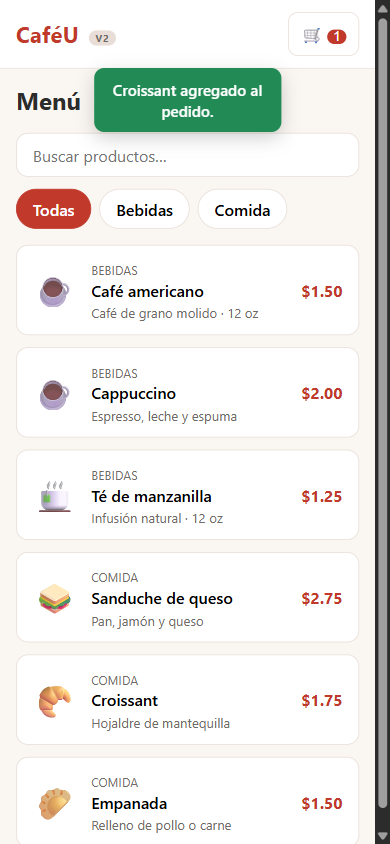
\includegraphics[width=0.47\textwidth]{imagenes/v2-aviso-agregado.png}
    \hfill
    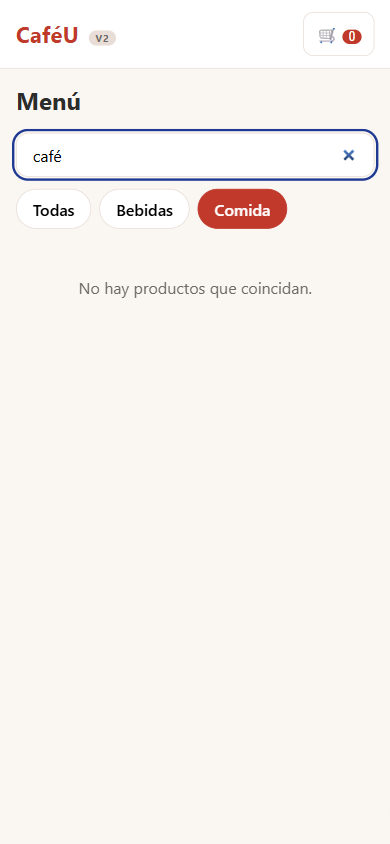
\includegraphics[width=0.47\textwidth]{imagenes/v2-busqueda-vacia.png}
    \caption{Aviso de «agregado al pedido» (izquierda) y estado vacío de la búsqueda con filtro activo (derecha).}
    \label{fig:v2-estado}
\end{figure}

\begin{figure}[H]
    \centering
    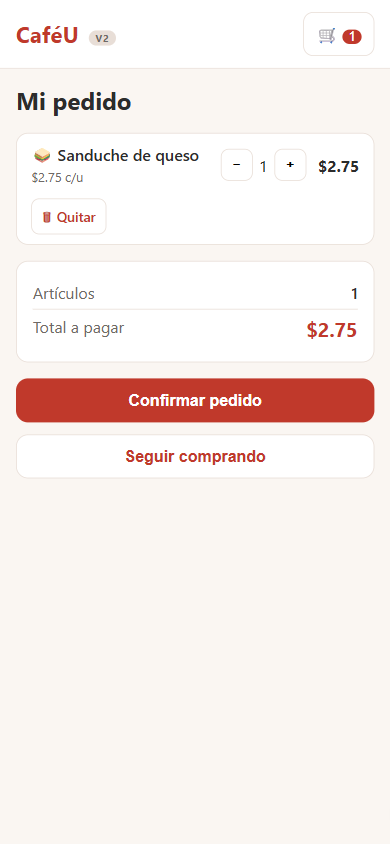
\includegraphics[width=0.47\textwidth]{imagenes/v2-pedido-quitar.png}
    \hfill
    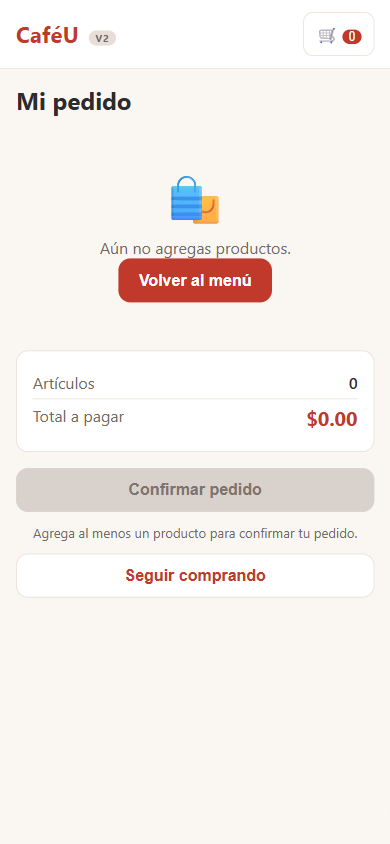
\includegraphics[width=0.47\textwidth]{imagenes/v2-confirmar-vacio.png}
    \caption{Botón «Quitar» en Mi pedido (izquierda) y confirmación bloqueada con pedido vacío (derecha).}
    \label{fig:v2-prevencion}
\end{figure}

\begin{figure}[H]
    \centering
    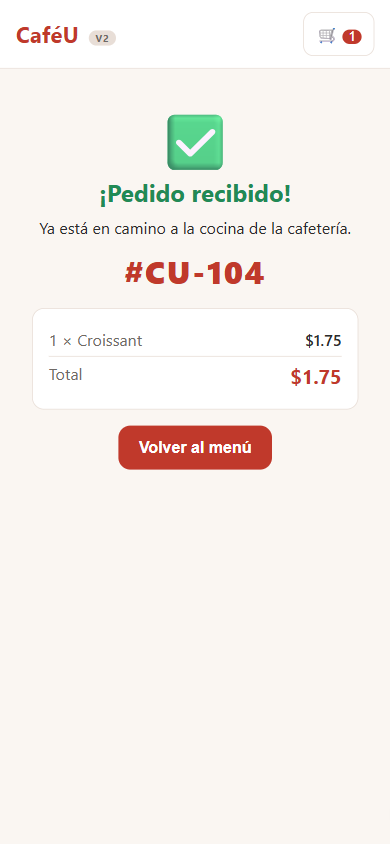
\includegraphics[width=0.5\textwidth]{imagenes/v2-confirmacion.png}
    \caption{Pantalla de confirmación con el código de retiro \texttt{\#CU-104}.}
    \label{fig:v2-confirmacion}
\end{figure}

\begin{figure}[H]
    \centering
    \includegraphics[width=0.3\textwidth]{imagenes/sesion-f3-p1.png}
    \hfill
    \includegraphics[width=0.3\textwidth]{imagenes/sesion-f3-p2.png}
    \hfill
    \includegraphics[width=0.3\textwidth]{imagenes/sesion-f3-p3.png}
    \caption{Evidencia anonimizada de las sesiones con P1, P2 y P3.}
    \label{fig:sesiones-f3}
\end{figure}

\subsubsection{Organización en GitHub}
Los entregables se encuentran en \texttt{ape6/Fase3-4/}: el README con las tablas de métricas, las cuatro evaluaciones heurísticas individuales, la evaluación consolidada, los registros P1--P3, los documentos de ajustes y protocolo y, en \texttt{docs/}, la matriz consolidada, la triangulación, los criterios técnicos, el backlog y las conclusiones. La carpeta \texttt{github/} contiene los nueve Issues redactados, con etiquetas, ramas, criterios de aceptación y matriz de revisión, listos para crearlos en el repositorio. El prototipo V2 está en \texttt{ape6/prototipo/} y el trabajo se mantiene en \url{https://github.com/Sax300-cpu/HCI-2026-G2}. Cada integrante crea su Issue y su Pull Request desde su cuenta, de modo que la autoría y la revisión queden registradas.

\subsection{Habilidades blandas empleadas en la práctica}
\begin{itemize}[leftmargin=1.5em, itemsep=2pt]
    \item[$\blacksquare$] Liderazgo
    \item[$\blacksquare$] Trabajo en equipo
    \item[$\blacksquare$] Comunicación asertiva
    \item[$\square$] La empatía
    \item[$\blacksquare$] Pensamiento crítico
    \item[$\square$] Flexibilidad
    \item[$\square$] La resolución de conflictos
    \item[$\square$] Adaptabilidad
    \item[$\blacksquare$] Responsabilidad
\end{itemize}

\subsection{Conclusiones}
\begin{itemize}[leftmargin=1.5em, itemsep=2pt]
    \item Los ajustes post-pilotaje fueron efectivos: T4 redujo su mediana de 24 s a 17 s, T6 pasó de 2/3 a 3/3 y el buscador normalizado resolvió T7 en 3/3.
    \item La eficacia se mantuvo alta (96,3~\% de éxito autónomo) y no se registraron errores críticos; los tres errores no críticos fueron recuperados por los participantes.
    \item La eficiencia cumplió todas las metas, con una mediana máxima de 19 s (T3) y un caso de 18 s en T8 que refleja el problema de recuperación de la búsqueda.
    \item La satisfacción fue alta (SUS 86,7), aunque el participante con menor puntaje (P2, 77,5) fue justamente quien no percibió el aviso y necesitó ayuda en T9.
    \item La inspección heurística y la prueba con usuarios aportaron hallazgos distintos: la heurística detectó cuatro riesgos que el recorrido feliz no disparó (H-03, H-05, H-06 y H-07) y los usuarios revelaron dos expectativas que ningún evaluador anticipó (H-08 y H-09).
    \item La triangulación confirma que los métodos no son intercambiables: la inspección cubrió el 77,8~\% de los hallazgos y los usuarios el 55,6~\%, con solo un tercio en común. Los tres hallazgos compartidos son los de mayor prioridad.
    \item La matriz consolidada cerró 9 hallazgos: 2 mayores, 4 menores y 3 cosméticos, sin ningún crítico. Los criterios C-01 a C-09 y el backlog de 22 horas permiten ejecutar las correcciones con evidencia y no por percepción.
    \item CaféU V2 es usable para completar el pedido, pero todavía no para que el usuario entienda lo que ocurre mientras lo hace: esa es la brecha que debe cerrar la siguiente versión.
\end{itemize}

\subsection{Recomendaciones}
\begin{itemize}[leftmargin=1.5em, itemsep=2pt]
    \item Mantener el reinicio F5 documentado y verificarlo antes de cada sesión para no contaminar los datos.
    \item Conservar la pista única estandarizada y registrar su uso, porque afecta la tasa de éxito autónomo.
    \item No declarar «usable» un prototipo solo porque las tareas se completan: los hallazgos de severidad 3 no impidieron terminar, pero sí afectaron la comprensión del estado.
    \item Ejecutar el backlog en el orden P1, P2, P3 y P4, re-ejecutando las tareas afectadas (T2, T8 y T9) al cerrar cada iteración.
    \item Mantener los criterios técnicos como condición de cierre de cada Issue y exigir la revisión de un integrante distinto del autor.
    \item Repetir la evaluación con cinco participantes después de las correcciones P1 y P2, incluyendo una tarea de exploración libre que pueda disparar H-03 y H-05.
\end{itemize}

\subsection{Referencias}
\begin{itemize}[leftmargin=1.5em, itemsep=2pt]
    \item Boehm, B. (1984). \textit{Software Engineering Economics}. Prentice Hall.
    \item Brooke, J. (1996). \textit{SUS: A quick and dirty usability scale}. En \textit{Usability Evaluation in Industry}.
    \item ISO. (2018). \textit{ISO 9241-11:2018 Ergonomics of human-system interaction --- Part 11: Usability: Definitions and concepts}. \href{https://www.iso.org/standard/63500.html}{iso.org/standard/63500.html}
    \item ISO. (2020). \textit{ISO 9241-110:2020 Ergonomics of human-system interaction --- Part 110: Dialogue principles}. \href{https://www.iso.org/standard/75258.html}{iso.org/standard/75258.html}
    \item Nielsen, J. (1994). \textit{10 Usability Heuristics for User Interface Design}. Nielsen Norman Group. \href{https://www.nngroup.com/articles/ten-usability-heuristics/}{nngroup.com}
    \item Nielsen, J. (1995). \textit{Severity Ratings for Usability Problems}. Nielsen Norman Group. \href{https://www.nngroup.com/articles/how-to-rate-the-severity-of-usability-problems/}{nngroup.com}
    \item W3C. (2023). \textit{Web Content Accessibility Guidelines (WCAG) 2.2}. \href{https://www.w3.org/TR/WCAG22/}{w3.org}
\end{itemize}

\end{document}
